\documentclass[aspectratio=169,10pt,t]{beamer}
% \usetheme[
% %%% options passed to the outer theme
% %    progressstyle=fixedCircCnt,   %either fixedCircCnt, movCircCnt, or corner
% %    rotationcw,          % change the rotation direction from counter-clockwise to clockwise
% %    shownavsym          % show the navigation symbols
%   ]{SDUsimple}
\usepackage{SDUtheme/beamerthemeSDUsimple}
% If you want to change the colors of the various elements in the theme, edit and uncomment the following lines
% Change the bar and sidebar colors:
%\setbeamercolor{SDUsimple}{fg=red!20,bg=red}
%\setbeamercolor{sidebar}{bg=red!20}
% Change the color of the structural elements:
%\setbeamercolor{structure}{fg=red}
% Change the frame title text color:
%\setbeamercolor{frametitle}{fg=blue}
% Change the normal text color background:
%\setbeamercolor{normal text}{fg=black,bg=gray!10}
% ... and you can of course change a lot more - see the beamer user manual.
\usepackage{color}
\usepackage{float}
\usepackage{dsfont}                         % Enables double stroke fonts
\usepackage{bm}
\usepackage[utf8]{inputenc}
\usepackage[english]{babel}
\usepackage[T1]{fontenc}
\usepackage{listings}
\usepackage{amsmath}
% Or whatever. Note that the encoding and the font should match. If T1
% does not look nice, try deleting the line with the fontenc.
\usepackage{helvet}
\usefonttheme{professionalfonts}

\newtheorem{algorithm}{Algorithm}
%\newtheorem{problem}{Problem}
\newtheorem{proposition}{Proposition}
% colored hyperlinks
\newcommand{\chref}[2]{%
	\href{#1}{{\usebeamercolor[bg]{SDUsimple}#2}}%
}

\title{Multivariate Analysis of Variance MANOVA}
\subtitle{Multivariate Statistic}
%\date{\today}
\date{ }

\author{
	Made by: \\
	\textbf{Lasse Gøransson, Marc Evald, Anne-Charlotte Poulsen \& Aske Møller}
}

% - Give the names in the same order as they appear in the paper.
% - Use the \inst{?} command only if the authors have different
%   affiliation. See the beamer manual for an example

\institute[
%  {\includegraphics[scale=0.2]{SDU_segl}}\\ %insert a company, department or university logo
SDU Robotics\\
The Maersk Mc-Kinney Moller Institute\\
University of Southern Denmark
] % optional - is placed in the bottom of the sidebar on every slide
{% is placed on the bottom of the title page
	SDU Robotics\\
	The Maersk Mc-Kinney Moller Institute\\
	University of Southern Denmark

	%there must be an empty line above this line - otherwise some unwanted space is added between the university and the country (I do not know why;( )
}

% specify a logo on the titlepage (you can specify additional logos an include them in
% institute command below
\pgfdeclareimage[height=0.5cm]{titlepagelogo}{SDUgraphics/SDU_logo_new} % placed on the title page
%\pgfdeclareimage[height=1.5cm]{titlepagelogo2}{SDUgraphics/SDU_logo_new} % placed on the title page
\titlegraphic{% is placed on the bottom of the title page
	\pgfuseimage{titlepagelogo}
	%  \hspace{1cm}\pgfuseimage{titlepagelogo2}
}

\begin{document}
% the titlepage
{\SDUwavesbg%
	\begin{frame}[plain,noframenumbering] % the plain option removes the header from the title page
		\titlepage
\end{frame}}
%%%%%%%%%%%%%%%%

\begin{frame}[t]
	\frametitle{Agenda}
	\framesubtitle{}

	\begin{itemize}
		\item Model
		\item MANOVA
		\item Model Check
		\item MANOVA2
	\end{itemize}

\end{frame}

\begin{frame}[t]
	\frametitle{Model}
	\begin{figure}[H]
		\includegraphics[scale=0.5]{images/modelManoca.png}
	\end{figure}
\end{frame}

\begin{frame}[t]
	\frametitle{MANOVA}
	\framesubtitle{1 factor}

	Assumptions:
	\begin{itemize}
		\item 
			\[
				X_{\ell,j} \sim N \left( \mu_\ell , \Sigma_\ell  \right) 
			\] 
		\item 
			\[
				\Sigma_1 = \Sigma_2 = \cdots = \Sigma_g
			\] 
		\item 
			\[
				\mu_\ell = \mu + \tau_\ell, \hspace{1cm} \sum^{g}_{\ell = 1} n_{\ell}\tau_{\ell}=0
			\] 
	\end{itemize}
	Hypothesis
	\[
		\begin{aligned}
			H_0 &: \forall \mu_\ell = \mu \hspace{1cm} \leftrightarrow 
			\hspace{1cm} \forall \tau_\ell = 0\\
			H_1 &: \exists \tau_\ell \neq 0
		\end{aligned}
	\] 

\end{frame}

\begin{frame}[t]
	\frametitle{Decomposition of variance}
	\[
		\begin{aligned}
			SST &=
			\sum^{g}_{\ell=1} 
			\sum^{n_{\ell}}_{j=1} 
			\left( X_{\ell,j}- \bar{X} \right) 
			\left( X_{\ell,j}- \bar{X} \right) ^{T}\\
			SSW &=
			\sum^{g}_{\ell=1} 
			\sum^{n_{\ell}}_{j=1} 
			\left( X_{\ell,j}- \bar{X}_{\ell} \right) 
			\left( X_{\ell,j}- \bar{X}_{\ell} \right) ^{T}\\
			SSB &=
			\sum^{g}_{\ell=1} 
			\sum^{n_\ell}_{j=1} 
			\left( \bar{X_{\ell}}- \bar{X} \right) 
			\left( \bar{X_{\ell}}- \bar{X} \right) ^{T}\\
		\end{aligned}
	\] 
	\vspace{1cm}
	\pause
	\[
		\Lambda ^{*} = \frac{|SSW|}{|SSB + SSW |} 
	\] 

\end{frame}

\begin{frame}[t]
	\frametitle{Illustration}
	\begin{figure}[H]
		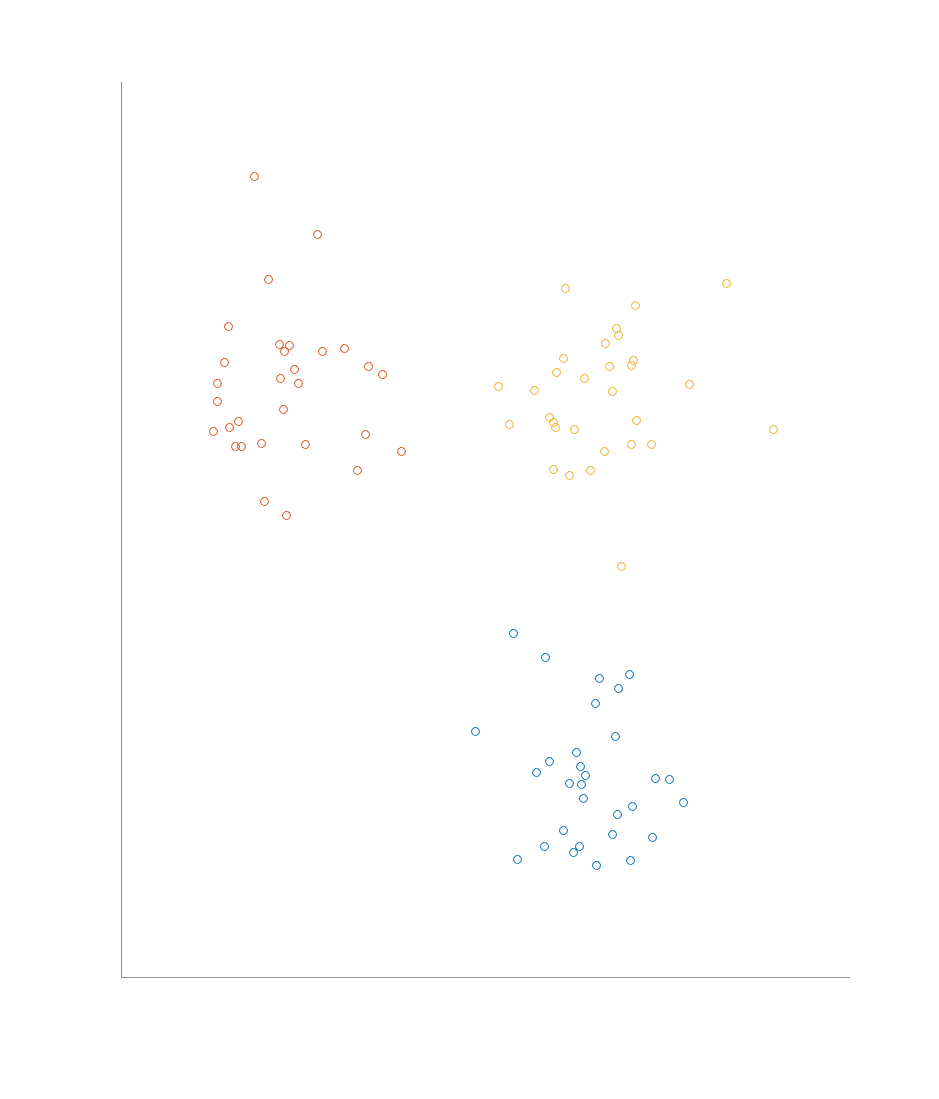
\includegraphics[scale=0.28]{clusters.png}
	\end{figure} 
\end{frame}
\begin{frame}[t]
	\frametitle{Exact Distributions of Wilks Lambda.}

	\begin{figure}[H]
		\centering
		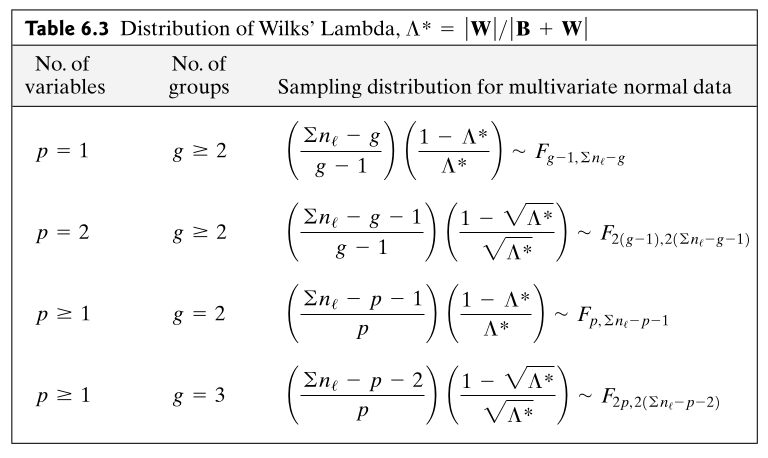
\includegraphics[scale=0.3]{images/1.png}
	\end{figure}
\end{frame}

\begin{frame}[t]
	\frametitle{Approximate distribution of Wilks Lambda.}
	\[
		-\left(n-1-\frac{p+g}{2}\right)ln\left( \Lambda^*\right) \sim \chi^2_{p(g-1)}
	\]  
\end{frame}

\begin{frame}[t]
	\frametitle{Pairwise CI's}
	\[
		\left[
			( \bar{X}_{ai} - \bar{X}_{bi}  ) 
			\pm t_{n-g},
			\frac{\alpha}{ \frac{pg(g-1)}{2} } \cdot 
			\sqrt{S_{wii} \cdot \left(  \frac{1}{n_a} + \frac{1}{n_b}  \right) }
	\right] , i = 1,...,p \land a,b = 1,...,g
	\] 

	\begin{figure}[H]
		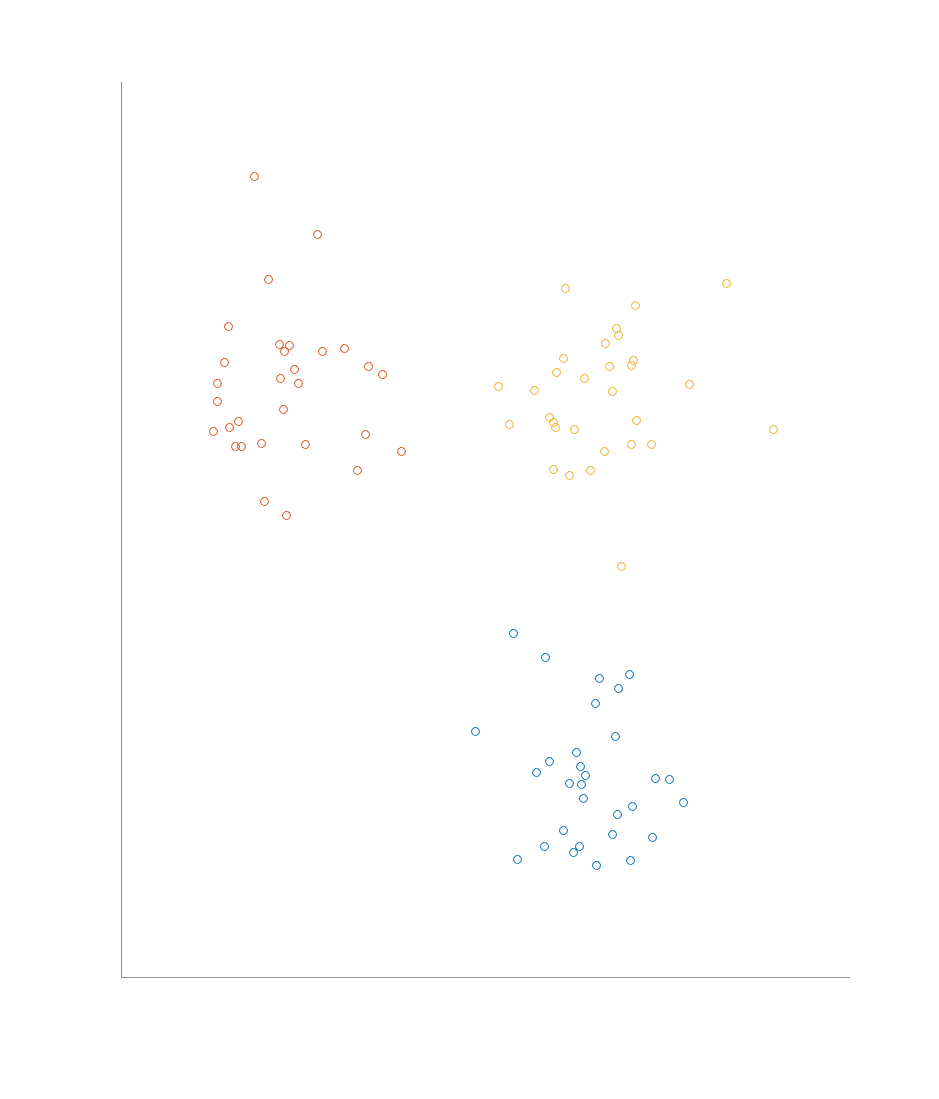
\includegraphics[scale=0.2]{clusters.png}
	\end{figure}
\end{frame}


\begin{frame}[t]
	\frametitle{Model Check}
	Hypothesis:
	\[
		\begin{aligned}
			H_0 &: \forall \Sigma_\ell = \Sigma\\
			H_1 &: \exists \Sigma_\ell \neq \Sigma
		\end{aligned}
	\] 

	Likelihood Ratio Test
	\[
		\Lambda = \frac{\underset{\Sigma}{max}L(\Sigma)}{\underset{\Sigma_1,\cdots,\Sigma_g}{max}L(\Sigma_1,\cdots,\Sigma_g)} 
	\] 
	\[
		-2\log\Lambda =  \left((n-g)\log|S_p| - \sum^{g}_{l=1}(n_l - 1) \log|S_l| \right) 
	\]
	Reject:
	\[
		-2c \cdot \log\Lambda > \chi^2_{p \frac{p+1}{2}, \alpha}
	\] 

\end{frame}


\begin{frame}[t]
	\frametitle{MANOVA2}

	Assumptions:
	\begin{itemize}
		\item 
			\[
				X_{\ell k,j} \sim N_{p}  \left( \mu_{\ell k}, \Sigma_{\ell k}  \right) 
			\] 
		\item 
			\[
				\forall \Sigma_{\ell k} = \Sigma
			\] 
		\item 
			\[
				\mu_{\ell k} = \mu + \tau_{\ell} + \beta_{k} + \gamma_{\ell k}
			\] 
	\end{itemize}

	Hypothesis\\
	\begin{centering}

		\begin{tabular}{ccc}
			$
			\begin{aligned}
				H_{0,\gamma} &: \forall \gamma_{\ell k} = 0\\
				H_{1,\gamma} &: \exists \gamma_{\ell k} \neq 0
			\end{aligned}
			$ & $
			\begin{aligned}
				H_{0,\tau} &: \forall \tau{\ell} = 0\\
				H_{1,\tau} &: \exists \tau{\ell} \neq 0
			\end{aligned}
			$	& $
			\begin{aligned}
				H_{0,\beta} &: \forall \beta_{k} = 0\\
				H_{1,\beta} &: \exists \beta_{k} \neq 0
			\end{aligned}
			$
		\end{tabular}
	\end{centering}
\end{frame}



\end{document}
